\documentclass[a4paper]{article}
\usepackage[slovene]{babel}
\usepackage[utf8]{inputenc}
\usepackage[T1]{fontenc}
\usepackage{graphicx}
\usepackage{marvosym}
\usepackage{amssymb,amsmath}
\title{Verjetnost sekanja konveksne podmnožice}
\author{Peter Dolenc, Jan Rems \\ Finančni praktikum \\ Finančna matematika, Fakulteta za matematiko in fiziko}
\date{2017}
\newtheorem{definicija}{Definicija}
\newtheorem{izrek}{Izrek}


\begin{document}
\title{%
  Verjetnost sekanja konveksne podmnožice -\\
   \large Poročilo dela \\}

\author{Peter Dolenc, Jan Rems}

\maketitle

\pagebreak

\section{Uvod}

\subsection{Generiranje premic}
Pri projektu se je izkazalo, da je zelo pomembno, kako generiramo naključne premice. Da dobimo željeni rezultat, namreč da je verjetnost sekanja tudi male krivulje enak razmerju obsegov obeh krivulj, je potrebno generirati par $(p, \theta)$ iz enakomerno zvezne porazdelitve, kjer $p$ predstavlja oddaljenost iz izhodišča in teče med $0$ in najbolj oddaljeno točko večje konveksne krivulje od izhodišča, $\theta$ pa predstavlja kot med premico in $x$-osjo ter teče med $0$ in $2\pi$. Matriko velikosti$n\times2$ s temi pari parametrov sva potem s pomožno funkcijo spremenila v matriko velikosti $n\times2$, kjer je prvi stolpec vseboval koeficiente $k$, drugi pa začetne vrednosti $n$ iz eksplicitnega zapisa premic $y=k\cdot x+n$. To nama je omogočilo, da sva določila daljice s krajišči izven večje krivulje, s katerimi sva sekala obe krivulji.

Poskusila sva tudi alternativno: generirala sva pare točk v večji konveksni množici in skozi njih potegnila premice. Izkazalo se je, da tak način generiranja premic ne pripelje do istega rezultata, saj je že za elipse v središču prišlo do velike napake. Da so premice generirane enakomerno glede na parametre $p$ in $\theta$ se je torej izkazalo za ključno.

\subsection{Generiranje konveksnih krivulj}
Pri generiranju konveksnih krivulj sva se odločila da iz enostavnejših konveksnih krivulj preideva na zahtevnejše in splošnejše primere. Začela sva z generiranjem elips, kjer je tudi notranja elipsa kocentrična. Nato sva obnašanje algoritma želela preveriti na primerih, kjer notranje krivulje niso nujno kocentrične, torej se nahajajo na poljubnem mestu znotraj zunanje krivulje. Zaradi olajšanja konstrukcije takih krrivulj sva se odločila za delo s krožnicami. Nazadnje pa sva zgenerirala še naključni oziroma poljubni konveksni krivulji. 

\subsubsection{Elipse}
Eksperimentalni del projekta je potekal v dveh fazah. V prvi sva najino hipotezo želela pokazati na enostavnejših konveksnih krivuljah - elipsah. Napisala sva funkcijo ``elipsa'', ki za vhodne podatke dobi parametra $xmax$ in $ymax$, ki določata največji možni števili $a$ in $b$, ki se pojavita v parametriziranem zapisu elipse $x=a \cos(t), y=b \sin(t), t\in [0, 2\pi)$. Kot izhod vrne dva poligona točk v obliki elipse z naključno izbranima parametroma $a \in (0, xmax)$ in $b \in (0, ymax)$ iz enakomerne zvezne porazdelitve za veliko elipso in $a_m \in (0, a)$ in $b_m \in (0, b)$ za malo elipso. V zadnjem koraku sva združili funkciji, ki generirata premice in elipsi ter dodala funkcijo, ki šteje presečišča med krivuljami. Za lažjo predstavo si oglejmo sliko 1:


\begin{figure}[h]
\centering
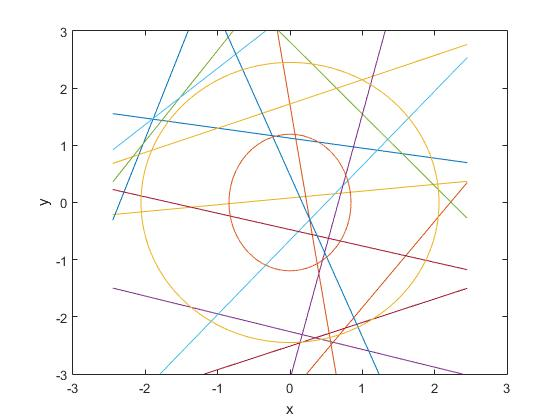
\includegraphics[width=60mm]{graf_primer.jpg}
\caption{Primer generiranih elips in premic \label{overflow}}
\end{figure} 

Na sliki 1 vidimo 2 elipsi generirani s funkcijo ``elipsa'' s parametroma $xmax=3$ in $ymax=3$ in 15 premic. V zadnjem koraku sva uporabilo funkcijo, ki šteje presečišča premic z obema elipsama ter število presečišč z manjšo krivuljo delila s številom presečišč z večjo. Rezultat sva primerjala z oceno razmerij obsega. 




Razmeroma zaneslijve rezultate sva dobila, če sva preko posameznega para elips generirala več kot 300 premic. Zato sva generirala 1000 parov elips in za vsak par 1000 premic, da sva lahko ocenila rezultate v povprečju. Povprečje absolutnih vrednosti razlike med razmerjem obsegov in razmerjem premic, ki sekajo eno in drugo krivuljo je bila 0.0125, če pa dovolimo predznačeno razliko, se je v povprečju zmanjšala na 0.000046 \footnote[1]{Celotna tabela rezultatov je dosegljiva na github repozitoriju}.

Zanimalo naju je tudi, kako hitra je konvergenca najine metode, oz. koliko premic je potrebno generirati za posamezen par elips, da bo rezultat točen. Rezultate sva dobila tako, da sva za vsak par elips primerjala absolutno razliko do točnega rezultata po vsakih 30 dodatnih premicah. Na vzorcu 100 elips je razmerje prikazano na grafu 1: 

\begin{figure}[h]
\centering
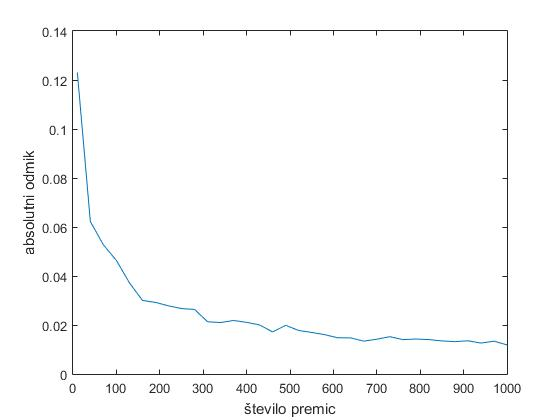
\includegraphics[width=90mm]{graf_elipsa2.jpg}
\caption{Graf napake v razmerju s številom premic \label{overflow}}
\end{figure} 

\subsubsection{Zamaknjene krožnice}

Za ponazoritev zamaknjenih krivulj sva se, iz praktičnih razlogov pri generiranju le-teh, odločila za krožnice. Funkciji "kroznica\_zamaknjena" sva podala parameter $rmax$, ki določa interval $(0,rmax)$ na katerem naključno določiva radij večjega kroga $r$. Nato znotraj kroga naključno generirava točko podano s parom $(k,fi)$, kjer je $k$ oddaljenost od izhodišča, $fi$ pa kot, ki ga oklepata abcisa in krajevni vektor do naše točke. Radij manjše krožnice $rm$ generirava naključno na intervalu $(0,(r-k))$. Nato krožnici parametrizirava, na podoben način kot elipsi. $x$ kordinate množice točk so podane kot vektor $x = r*cos(t)$, $y$ kordinate pa kot vektor $y = r*sin(t)$, kjer je t vektor točk med 0 in $2\pi$ z razmikom 0.05. Manjšo krožnico parametrizirava na podoben način.  Funkcija torej vrne matriki, kjer v vsaki stolpca predstavljata $x$ in $y$ kordinate množice točk, ki krožnici določajo. 

\subsubsection{Splošna  konveksna krivulja}
Splošni konveksni krivulji generirava s pomočjo dveh funkcij: "random\_konveksna" in "notranja\_konveksna". Prva dobi za parameter$j$, ki ponazarja število naključnih točk, ki jih bo funkcija generirala. Točke so podane z dvema vektorjema $a$ in $b$ dolžine $j$, ki vsebujeta naključna štvila na intevalu $[-0.5,0,5]$. Nato na teh dveh vektorjih pokličemo vgrajeno funkcijo "convhull", ki za podano množico točk, vrne vektor indeksov točk $h$, ki razpenjajo  najmanjšo konveksno ovojnico, ki vsebuje vse točke, podane v argumentu. Funkcija torej na koncu vrne trojico vektorjev $a,b$ in $h$. FUnkcija "notranja\_konveksna" pa deluje tako, da najprej iz vektorjev $a$ in $b$, ki ju vrne"random\_konveksna" odstrani elemente na mestih, ki so podani v vektorju $h$. Nato izmed preostalih točk naključno izbere 40% le-teh in jih vrne kot vektorja $a1$ in $b1$. Na dani množici točk ponovno pokličeva funkcijo "convhul" rezultat pa shranimo kot $l$. Funkcija  "notranja\_konveksna" vrne trojico "a1,a2$ in $l$. Primer generiranih splošnih konveksnih krivulj je prikazan v grafu spodaj.


\begin{figure}[h]
\centering
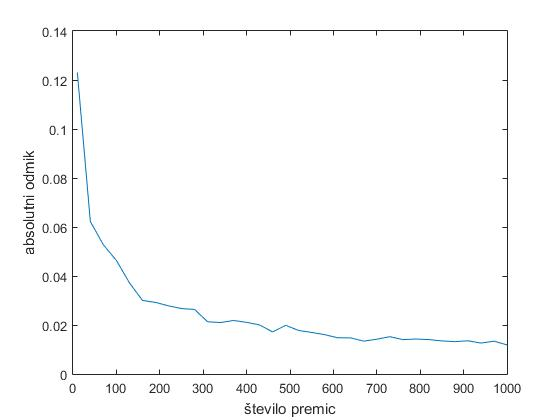
\includegraphics[width=90mm]{graf_elipsa2.jpg}
\caption{Graf napake v razmerju s številom premic \label{overflow}}
\end{figure} 


\subsection{Al





\end{document}

Iz grafa je razvidno, da se z večanjem premic vedno bolj približujemo pravemu rezultatu, vendar je konvergenca počasna. 